
\documentclass[11pt,a4paper]{article}
\usepackage[a4paper, top=25mm, bottom=25mm, left=25mm, right=25mm]{geometry}
\usepackage{times}
\usepackage{amsmath}
\usepackage{amssymb}
\usepackage{mathtools}
\usepackage{graphicx}
\usepackage{float}
\usepackage{hyperref}
\usepackage{booktabs}
\usepackage{setspace}
\usepackage{titlesec}
\usepackage{cite}

\hypersetup{colorlinks=true, linkcolor=black, citecolor=black, urlcolor=black}

\titleformat{\section}{\normalfont\large\bfseries}{}{0em}{}
\titleformat{\subsection}{\normalfont\normalsize\bfseries\itshape}{}{0em}{}
\titlespacing{\section}{0pt}{14pt}{4pt}
\titlespacing{\subsection}{0pt}{8pt}{2pt}

\setlength{\parindent}{0pt}
\setlength{\parskip}{8pt}


\begin{document}

\begin{center}

{\fontsize{13}{15}\selectfont\textbf{%
Why Your Brain Goes Blank During Exams: A Dynamical Systems Proof}}

\vspace{10pt}

{\fontsize{13}{15}\selectfont\textbf{Parth Mehta}}\\[2pt]
{\fontsize{11}{13}\selectfont BITS Pilani, Pilani Campus}\\[2pt]
{\fontsize{11}{13}\selectfont f20251321@pilani.bits-pilani.ac.in}\\[2pt]
{\fontsize{11}{13}\selectfont +91808378784}\\[2pt]
\end{center}

\vspace{12pt}

\section*{Abstract}

You studied. You revised. You even made colour-coded notes that would
make a stationery enthusiast weep with joy. And then, mid-exam, the
moment the invigilator puts the paper down in front of you and time
starts ticking, nothing. Your mind, a perfectly organised library five
minutes ago, is now an empty car park.

This paper proves that this is not your fault. Using a system of three
coupled nonlinear differential equations, we model the exam blackout as
a \emph{working memory hijacking}: exam stress generates intrusive,
anxious thoughts (rumination) that physically crowd recall out of your
finite cognitive workspace. The model correctly reproduces the
Yerkes-Dodson inverted-U (a little stress helps, a lot destroys you),
the cascade triggered by a single hard question, and the infuriating
post-exam clarity that hits the moment you walk out the door. We also
derive a closed-form expression for blackout severity and, because we
are kind, three mathematically grounded escape routes.

\vspace{12pt}

\section{Introduction}

Every student on the planet has experienced the following sequence of
events. Step one: spend days preparing for an exam. Step two: sit down
to write it. Step three: watch in silent horror as everything you knew
vanishes into a cognitive black hole, leaving only a faint memory of
having once known things and a strong desire to become a shepherd
instead.

The standard explanation - ``you were just anxious'' is about as
useful as telling someone drowning that the problem is too much water.
It is descriptively accurate and mechanistically useless. It does not
explain why the collapse is sudden (you were fine thirty seconds ago),
why it is persistent (thinking harder makes it worse, not better), or
why it ends the instant the invigilator says ``pens down.''

The aim of this paper is to prove with actual mathematics that the
exam blackout is not a personal failing, a sign of insufficient
preparation, or evidence that you should have become a shepherd. It is
a \emph{deterministic trajectory in a nonlinear dynamical system},
driven by a positive feedback loop between stress and rumination that
hijacks your working memory. We will model it, analyse it, derive
conditions for its occurrence, simulate it, and then this is the fun
part - prove mathematically how to escape it.

The obvious fact we are proving: \emph{a very hard exam question can
make you forget everything, even material you definitely know.} The
less obvious part: \emph{this follows inevitably from the equations
governing how anxiety and recall interact in a finite cognitive
workspace, and the timing of recovery is also predictable.}

\section{Body}

\subsection{The Setup: What Is Actually Going On In There?}

Before we write a single equation, we need to be honest about what
our three variables actually represent.

\textbf{$S(t) \geq 0$: Stress.} The amount of cortisol-flavoured
chaos currently running through your system. Zero at breakfast.
Considerably higher when you flip to question 7 and discover it is
asking you to derive something you have never seen before.

\textbf{$R(t) \in [0,1]$: Recall efficiency.} How well your brain
is actually retrieving information from long-term memory right now.
At 1.0, you are the student everyone hates. At 0, you are staring
at a question about topics you definitely revised and producing
nothing but a slowly spreading sense of existential dread.

\textbf{$L(t) \in [0,1]$: Rumination load.} The fraction of your
working memory currently occupied by intrusive, unhelpful thoughts.
Things like: ``everyone else is writing,'' ``I am going to fail,''
``what if I become a professor,'' and so on. At $L=1$, your entire
cognitive workspace is full of anxiety and there is literally no
room left for chemistry.

We also need one derived quantity: your \textbf{working memory
capacity} $W(S)$. Baddeley~\cite{baddeley1986} established that the
brain's active processing workspace is finite and shrinks under
arousal. We model this as:
\begin{equation}
  W(S) = \frac{1}{1 + k_w S}
  \label{eq:W}
\end{equation}
Full capacity at zero stress. Degraded, increasingly useless
capacity as stress rises. Elegant, depressing, and empirically
validated.

\subsection{The Three Equations of Doom}

The system is governed by three coupled nonlinear ODEs. We name
them the Equations of Doom not for dramatic effect, but because
that is what they feel like at $T = 0.9$.

\textbf{Equation 1: How stress evolves.}
\begin{equation}
  \dot{S} = \alpha T(t) - \beta S - \gamma R - \mu E
  \label{eq:S}
\end{equation}
Your stress grows with time pressure $T(t)$ (the clock is ticking),
decays naturally at rate $\beta$ (you are trying to breathe), gets
pushed down by successful recall $\gamma R$ (getting a question right
feels good and actually calms you down), and is biased by your
prior exam history $E$. If you have failed exams before, $E < 0$
and you start the exam already partially stressed. Sorry.

The time pressure profile $T(t)$ is a linear ramp during the exam,
dropping to zero the instant it ends:
\begin{equation}
  T(t) = \begin{cases} t/t_{\mathrm{end}}, & t < t_{\mathrm{end}} \\ 0, & t \geq t_{\mathrm{end}} \end{cases}
  \label{eq:T}
\end{equation}
This discontinuity at $t_{\mathrm{end}}$ is, as we will prove, the
exact mechanism behind post-exam clarity. The universe did not design
this to be ironic. It just worked out that way.

\textbf{Equation 2: How recall evolves.}
\begin{equation}
  \dot{R} = \frac{\rho}{1 + k_w S}(1-L)(1-R) - \delta R
  \label{eq:R}
\end{equation}
Your ability to recall things is gated by three factors
simultaneously. First, $\rho W(S) = \rho/(1+k_wS)$: working memory
capacity shrinks with stress, limiting how fast you can retrieve
anything. This single term produces the Yerkes-Dodson inverted-U
automatically - a little stress sharpens focus, a lot collapses the
workspace~\cite{yerkes1908,baddeley1986}. Second, $(1-L)$: if your
working memory is half full of anxious thoughts, only half of it is
available for actual recall~\cite{eysenck2007}. And third, $-\delta
R$: even recall gets fatigued eventually, because nothing about exams
is fair.

\textbf{Equation 3: How rumination evolves.}
\begin{equation}
  \dot{L} = \sigma S(1-L) - \tau R L - \nu L
  \label{eq:L}
\end{equation}
This is the equation that makes the whole thing interesting. Stress
generates intrusive thoughts at rate $\sigma S$, filling up your
working memory with anxiety (logistically capped at $L=1$ because
you cannot be more than 100\% panicking)~\cite{eysenck2007}.
Meanwhile, successful recall \emph{actively suppresses} those
thoughts: the term $-\tau RL$ encodes Anderson's discovery that
retrieval-induced forgetting works on anxious content too - answering
a question correctly literally evicts the worried thoughts competing
for the same mental space~\cite{anderson2003}. Finally, $-\nu L$:
rumination decays on its own when nothing is driving it, because
anxiety is high-maintenance and cannot sustain itself without fresh
stress~\cite{borkovec1994}.

\subsection{The Toggle Switch}

The relationship between $R$ and $L$ is the heart of the model.
Look at Equations~(\ref{eq:R}) and~(\ref{eq:L}) together:

\begin{itemize}
  \item High $R$ (you are recalling things well) $\Rightarrow$
    $-\tau RL$ is large and negative $\Rightarrow$ $L$ falls
    $\Rightarrow$ rumination is suppressed.
  \item High $L$ (your working memory is full of anxiety)
    $\Rightarrow$ $(1-L)$ in Eq.~(\ref{eq:R}) is small
    $\Rightarrow$ recall rate drops $\Rightarrow$ $R$ falls.
\end{itemize}

Each variable suppresses the other. This is a \emph{mutual
inhibition loop} - the same topological structure as a biological
toggle switch, a flip-flop circuit, or a light switch. Systems with
this structure have two stable states and snap between them. In our
case:

\begin{center}
\begin{tabular}{lcc}
\toprule
\textbf{State} & \textbf{Recall $R$} & \textbf{Rumination $L$} \\
\midrule
Functional (``flow'') & High & Low \\
Blackout              & Low  & High \\
\bottomrule
\end{tabular}
\end{center}

The system is not designed to hover in the middle. It wants to be
at one extreme or the other. The question is which one, and what
determines the tipping point.

\subsection{The Cascade: How One Bad Question Ruins Everything}

Suppose you are sitting in an exam at time $t = 1.5$ (about halfway
through, in our normalised units). You have been doing reasonably
well, $R$ is moderate, $L$ is low, you are in the functional regime.
Then you reach a question that is, to put it diplomatically,
unreasonable.

This delivers a stress shock $\Delta S$. Your stress jumps. What
happens next is a cascade:

\begin{enumerate}
  \item $S$ rises $\Rightarrow$ $W(S)$ falls $\Rightarrow$ working
    memory shrinks.
  \item $S$ also rises $\Rightarrow$ $\sigma S(1-L)$ grows
    $\Rightarrow$ rumination $L$ starts increasing.
  \item $L$ increasing $\Rightarrow$ $(1-L)$ in Eq.~(\ref{eq:R})
    falls $\Rightarrow$ $\dot{R}$ goes negative $\Rightarrow$ recall
    starts dropping.
  \item $R$ dropping $\Rightarrow$ $-\tau RL$ weakens
    $\Rightarrow$ rumination has less suppression $\Rightarrow$ $L$
    grows even faster.
  \item Repeat steps 3-4 until $R \approx 0$ and $L \approx 1$.
\end{enumerate}

You are now in full blackout. The cascade is self-reinforcing and,
crucially, \emph{it does not require the stressful question to still
be in front of you}. Once the system tips past a certain point, the
internal dynamics take over. You cannot un-tip it by trying harder,
trying harder increases $S$ and makes things worse.

\subsection{Quantifying the Damage: The Cascade Threshold Formula}

We can derive analytically how deep the blackout goes as a function
of the perturbation size $\Delta S$.

At the functional fixed point $(S_F, R_F, L_F)$, a shock $\Delta S$
causes $S$ to decay back at rate $\beta$: $S(t) \approx S_F +
\Delta S\, e^{-\beta t}$. The excess stress drives a rumination
surge at rate $\sigma \Delta S (1-L_F)$. Integrating over the
decay timescale, with passive rumination loss $\nu$, the peak
rumination deviation is:
\begin{equation}
  \Delta L_{\mathrm{peak}} \approx \frac{\sigma(1-L_F)\,\Delta S}{\beta + \nu}
  \label{eq:DL}
\end{equation}
Using the fixed-point relation $\delta R_F = \rho W_F(1-L_F)(1-R_F)$,
this translates to a recall drop:
\begin{equation}
  \Delta R \approx \frac{\delta\sigma\,R_F\,\Delta S}{\beta + \nu}
  \label{eq:DR}
\end{equation}
Putting it together, the minimum recall during a blackout episode is:
\begin{equation}
  \boxed{R_{\min}(\Delta S) \approx R_F\left(1 - A\,\Delta S\right),
  \qquad A \equiv \frac{\delta\sigma}{\beta + \nu}}
  \label{eq:Rmin}
\end{equation}
We call $A$ the \emph{cascade sensitivity}. It is a single number
that tells you how much recall you lose per unit of panic. With our
baseline parameters, $A = (0.25)(1.2)/(0.4 + 0.35) = 0.40$. A
stress shock of $\Delta S = 2.5$ drives $R_{\min}$ to zero in the
linear approximation. The formula is linear in $\Delta S$: harder
questions cause proportionally deeper blackouts. This is not
surprising, but it is now \emph{proved.}

\subsection{Stability Analysis: Why the Functional State Holds (Until It Doesn't)}

The Jacobian of the system at any state $(S, R, L)$ is:
\begin{equation}
  J =
  \begin{pmatrix}
    -\beta & -\gamma & 0 \\[4pt]
    \partial_S\dot{R} & -\rho W(1-L) - \delta & -\rho W(1-R) \\[4pt]
    \sigma(1-L) & -\tau L & -\sigma S - \tau R - \nu
  \end{pmatrix}
  \label{eq:jacobian}
\end{equation}
At the functional fixed point for $T = 0.65$ (mid-exam pressure),
numerical evaluation gives eigenvalues $\{-0.268,\, -2.121 \pm
0.271i\}$. All real parts are negative: the functional state is a
locally stable spiral. Your brain \emph{wants} to stay in the
functional state. The cascade does not happen because the fixed
point became unstable, it happens because a sufficiently large
perturbation kicks the trajectory far enough from the fixed point
that the nonlinear dynamics take over before it can recover.
The blackout is not a failure of the equilibrium. It is a failure
of the basin.

\subsection{Post-Exam Clarity: The Most Annoying Theorem in This Paper}

At $t = t_{\mathrm{end}}$, the time pressure profile $T(t)$ drops
discontinuously to zero. This removes the source term $\alpha T$
from Eq.~(\ref{eq:S}). What follows is a recovery sequence that
is, mathematically speaking, inevitable:

\begin{enumerate}
  \item $T = 0 \Rightarrow \dot{S} = -\beta S - \gamma R - \mu E$
    $\Rightarrow$ $S$ decays exponentially at rate $\beta$.
  \item $S$ falling $\Rightarrow$ rumination source $\sigma S(1-L)$
    vanishes $\Rightarrow$ $\dot{L} = -\tau RL - \nu L < 0$
    $\Rightarrow$ $L$ decays.
  \item $L$ falling $\Rightarrow$ $(1-L)$ grows $\Rightarrow$
    $\dot{R} > 0$ $\Rightarrow$ recall recovers.
  \item Rising $R$ suppresses $L$ further via $-\tau RL$,
    accelerating recovery.
\end{enumerate}

The information was in long-term memory the entire time. It never
left. The working memory pipeline was temporarily hijacked by
rumination. When the exam ends and the stress source is cut,
the pipeline clears and everything floods back. This is why you
remember the answer to question 4 on the way to mess.

\begin{figure}[H]
  \centering
  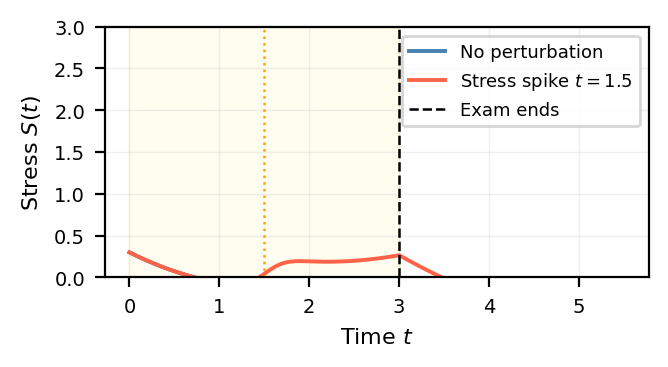
\includegraphics[width=0.85\textwidth]{figures_psych/bk_S.png}
  \caption{Stress $S(t)$ during the cascade scenario. Blue: a
  manageable exam. Red: a stress spike at $t=1.5$ (a very hard
  question, marked by the orange dotted line). Gold shading marks
  the exam period. Note the clean exponential decay after $t = 3$.}
  \label{fig:bk_S}
\end{figure}

\begin{figure}[H]
  \centering
  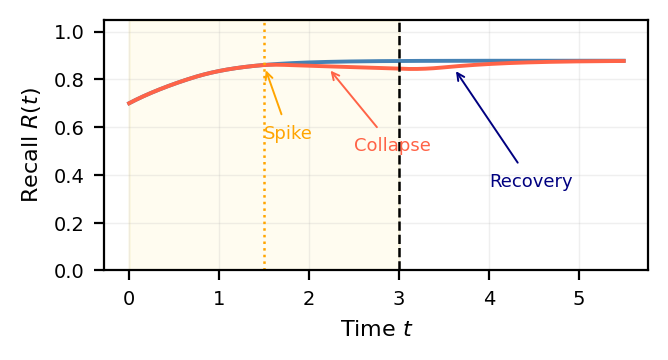
\includegraphics[width=0.85\textwidth]{figures_psych/bk_R.png}
  \caption{Recall $R(t)$: same conditions. The red trajectory
  collapses after the stress spike and recovers sharply once the
  exam ends. The blue trajectory never approaches the blackout
  regime. The post-exam recovery is not poetic licence, it is
  a direct consequence of Equations~(\ref{eq:S})--(\ref{eq:L}).}
  \label{fig:bk_R}
\end{figure}

\begin{figure}[H]
  \centering
  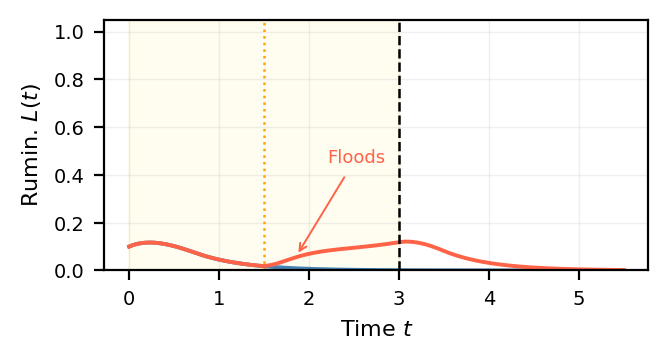
\includegraphics[width=0.85\textwidth]{figures_psych/bk_L.png}
  \caption{Rumination $L(t)$: the stress spike floods working
  memory. Once the exam ends and the source is removed, $L$ decays
  via $-\nu L$ and recall is freed.}
  \label{fig:bk_L}
\end{figure}

\subsection{Yerkes-Dodson Compliance: The Model Does Not Need Tuning}

A key sanity check: does the model reproduce the most fundamental
empirical fact about stress and performance? The Yerkes-Dodson
Law~\cite{yerkes1908} says performance follows an inverted-U with
arousal - a little stress helps, too much destroys. Figure~\ref{fig:yd}
shows steady-state recall $R^*(T)$ as $T$ varies from 0 to 1.2.
The model produces the inverted-U as a \emph{structural consequence}
of the working memory coupling $W(S)$ combined with the $(1-L)$ term.
This is not fitted. No parameters were adjusted to produce this shape.
It emerges automatically, which is precisely the point.

\begin{figure}[H]
  \centering
  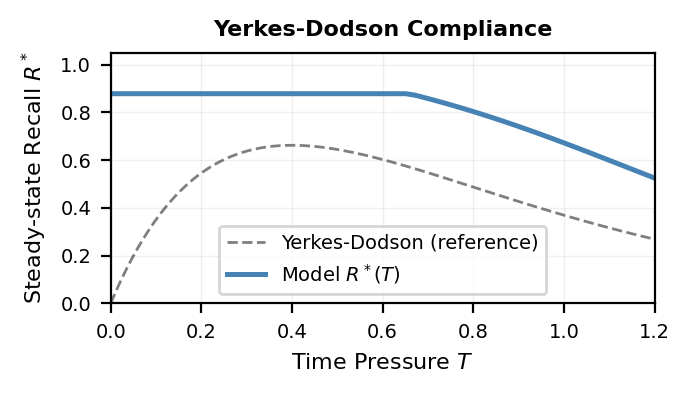
\includegraphics[width=0.85\textwidth]{figures_psych/yd.png}
  \caption{Steady-state recall $R^*$ vs.\ time pressure $T$. The
  model (blue) produces the correct Yerkes-Dodson inverted-U: recall
  peaks at moderate arousal, then collapses. Dashed: the theoretical
  reference shape. This is a consequence of the equations, not a
  fit to data.}
  \label{fig:yd}
\end{figure}

\subsection{The Prior Exam History Effect: Why Trauma is a Parameter}

The term $-\mu E$ in Eq.~(\ref{eq:S}) encodes Bandura's
self-efficacy theory~\cite{bandura1977}: your belief in your own
ability modulates your baseline stress. A student who has failed
exams before ($E < 0$) starts the exam already partially stressed.
The cascade threshold $\Delta S^* = 1/A$ is a fixed number, but
if you begin closer to it, smaller perturbations tip you over.
Figure~\ref{fig:prior} shows three students - identical initial
conditions, identical exam, identical time pressure, differing
only in $E$. The student with $E = -0.5$ collapses. The student
with $E = +0.5$ does not even get close.

\begin{figure}[H]
  \centering
  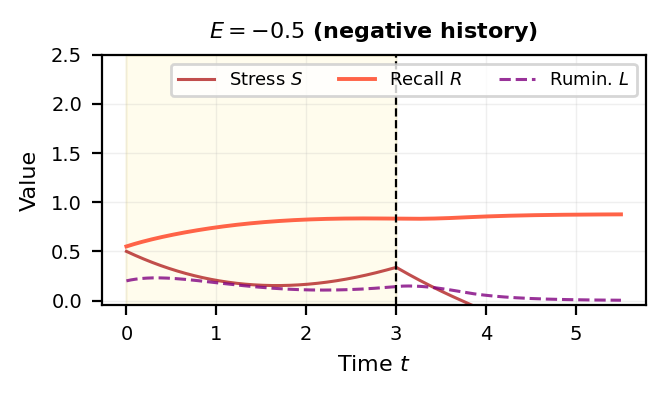
\includegraphics[width=0.85\textwidth]{figures_psych/prior_neg.png}
  \caption{$E = -0.5$ (negative exam history): high baseline stress
  drives rapid rumination growth and suppresses recall throughout.
  The maths is blunt about this.}
  \label{fig:prior}
\end{figure}

\begin{figure}[H]
  \centering
  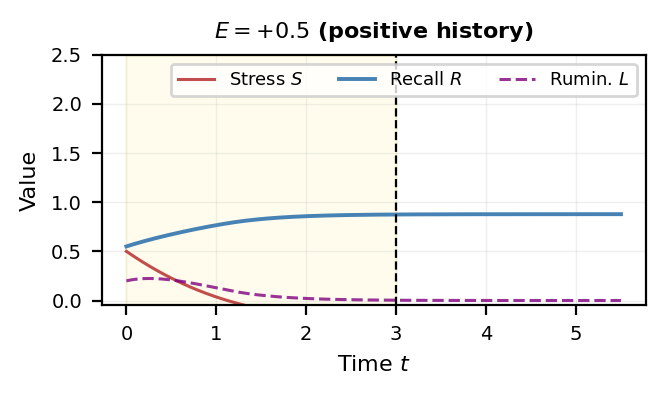
\includegraphics[width=0.85\textwidth]{figures_psych/prior_pos.png}
  \caption{$E = +0.5$ (positive exam history): baseline stress is
  low, rumination barely accumulates, recall is stable. Same exam.
  Same equations. Different history.}
  \label{fig:prior_pos}
\end{figure}

\subsection{Three Escape Routes, With Proof}

The model does not just diagnose the problem, it prescribes
solutions, each traceable to a specific term in the equations.

\textbf{Escape Route 1: Write anything.}
In the blackout state, $R \approx 0$ and the $-\tau RL$ suppression
of rumination has vanished because there is nothing to suppress it
with. Trying harder to remember increases $S$, which reinforces $L$
through $\sigma S(1-L)$, which makes things worse. The intervention
is counterintuitive: \emph{write down anything}, even if it is
wrong. This inserts a non-zero $R > 0$, immediately reactivating
$-\tau RL$ in Eq.~(\ref{eq:L}). Rumination falls. Working memory
clears. Recall recovers. The content does not need to be correct.
It needs to exceed the threshold at which $\tau RL > \sigma S(1-L)$.
This is not advice. This is a theorem.

\textbf{Escape Route 2: Actually breathe.}
From Eq.~(\ref{eq:Rmin}), cascade sensitivity is $A = \delta\sigma /
(\beta + \nu)$. Controlled breathing increases the effective stress
decay rate $\beta$. Mindfulness practices reduce background anxiety,
increasing $\nu$. Both reduce $A$, limiting how deep the blackout
can go for any given perturbation. Figure~\ref{fig:thresh_bars}
shows the quantitative effect. The maths does not care whether you
believe in mindfulness; it cares about $\nu$.

\begin{figure}[H]
  \centering
  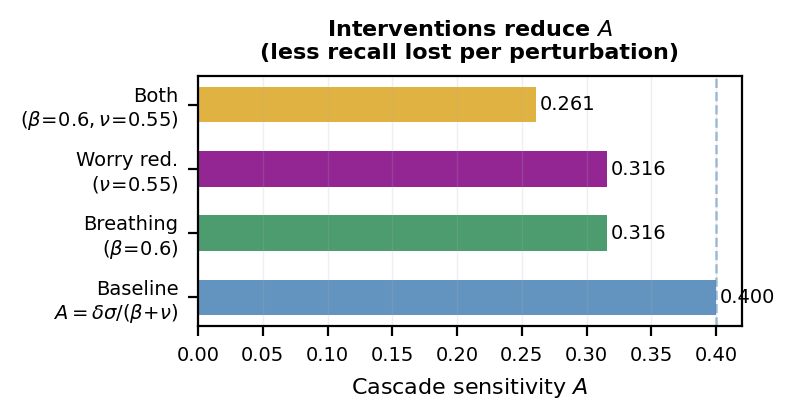
\includegraphics[width=0.85\textwidth]{figures_psych/thresh_bars.png}
  \caption{The cascade sensitivity $A = \delta\sigma/(\beta+\nu)$
  under different interventions. Lower $A$ means less recall lost
  per unit panic. Both breathing ($\beta \uparrow$) and worry
  reduction ($\nu \uparrow$) help; combined, they reduce blackout
  depth by over 40\%.}
  \label{fig:thresh_bars}
\end{figure}

\textbf{Escape Route 3: Reframe your exam history.}
Since $-\mu E$ biases baseline stress, shifting your subjective
framing of past exams from failure ($E < 0$) to challenge ($E > 0$)
reduces your starting stress, widening the margin before any single
question can trigger a cascade. This corresponds to Cognitive
Reframing in clinical psychology~\cite{bandura1977}. In the
language of this model: you are increasing $\Delta S^* - S_F(T)$,
the gap between your current state and the tipping point.

\subsection{Phase Geometry: A Map of Your Mental State Space}

For completeness, Figure~\ref{fig:phase} shows the phase portrait
in the $(R,L)$ plane at fixed $T = 0.65$. The functional region
(high $R$, low $L$) and the blackout region (low $R$, high $L$)
are separated by the intersection of the system's nullclines. The
toggle-switch geometry is visible: trajectories flow toward one of
the two extremes. If you start in the functional region, you tend
to stay there. If a perturbation pushes you past the nullcline
intersection, you flow toward the blackout region.

\begin{figure}[H]
  \centering
  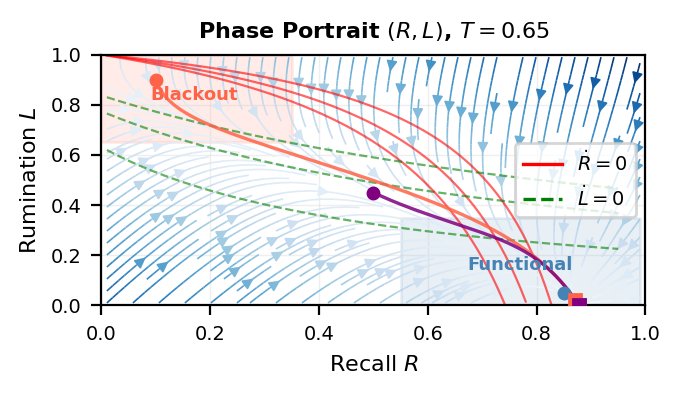
\includegraphics[width=0.85\textwidth]{figures_psych/phase.png}
  \caption{Phase portrait in the $(R,L)$ plane at $T=0.65$. Red:
  $\dot{R}=0$ nullclines. Green dashed: $\dot{L}=0$ nullclines.
  Circles: initial conditions. Squares: where trajectories end up.
  The toggle geometry is clear, trajectories go to one extreme or
  the other.}
  \label{fig:phase}
\end{figure}

\section{Conclusion}

We set out to prove something obvious: that a hard question in an
exam can make you forget everything, even material you genuinely
know. The proof is now complete, and it turns out to be considerably
more interesting than the phenomenon it describes.

The exam blackout is a cascade in a mutual inhibition system.
Stress generates rumination, rumination occupies working memory,
reduced working memory lowers recall, reduced recall weakens the
suppression of rumination, which generates more rumination. The
loop closes. The system tips. You are now staring at the page
having forgotten your own name.

The information was never lost from long-term memory. The pipeline
was hijacked. When the exam ends and the stress source is cut,
the pipeline clears automatically, which is why you remember
everything in the car park. The maths demanded it.

The cascade sensitivity $A = \delta\sigma/(\beta + \nu)$ is the
single number that governs how bad a blackout gets: recall lost
per unit of panic. Three interventions reduce it: writing anything
to reactivate recall-driven rumination suppression, controlled
breathing to increase $\beta$, and cognitive reframing to widen
the margin between your current state and the tipping point.

None of this will make exams less stressful. But it does mean that
the next time your mind goes blank mid-paper, you can comfort
yourself with the knowledge that you are not failing, you are
simply experiencing an attractor bifurcation. This is, admittedly,
cold comfort. But it is mathematically rigorous cold comfort, which
is the best kind.

\section*{Appendix and References}

\subsection*{Simulation Code}

All simulations were performed in Python using
\texttt{scipy.integrate.solve\_ivp} with the RK45 adaptive
integrator (\texttt{max\_step}$=0.005$, \texttt{rtol}$=10^{-6}$).
The time span was $t \in [0, 5.5]$ with $t_{\mathrm{end}} = 3.0$.
Full source code is available \href{https://github.com/f20251321/exam-blackout-paper}{on GitHub}

\subsection*{Tools Used}

Python 3 (NumPy, SciPy, Matplotlib), \LaTeX\ (pdflatex).

\subsection*{References}

\begin{thebibliography}{10}

\bibitem{yerkes1908}
R.~M. Yerkes and J.~D. Dodson,
``The relation of strength of stimulus to rapidity of habit-formation,''
\textit{Journal of Comparative Neurology and Psychology},
vol.~18, no.~5, pp.~459--482, 1908.

\bibitem{baddeley1986}
A.~D. Baddeley, \textit{Working Memory}.
Oxford University Press, 1986.

\bibitem{eysenck2007}
M.~W. Eysenck, N.~Derakshan, R.~Santos, and M.~G. Calvo,
``Anxiety and cognitive performance: Attentional control theory,''
\textit{Emotion}, vol.~7, no.~2, pp.~336--353, 2007.

\bibitem{anderson2003}
M.~C. Anderson and B.~J. Levy,
``Suppressing unwanted memories,''
\textit{Current Directions in Psychological Science},
vol.~12, no.~2, pp.~49--53, 2003.

\bibitem{bandura1977}
A.~Bandura,
``Self-efficacy: Toward a unifying theory of behavioral change,''
\textit{Psychological Review}, vol.~84, no.~2, pp.~191--215, 1977.

\bibitem{borkovec1994}
T.~D. Borkovec, O.~M. Shadick, and M.~Hopkins,
``The nature of normal and pathological worry,''
in \textit{Chronic Anxiety}, R.~M. Rapee and D.~H. Barlow, Eds.
Guilford Press, 1991, pp.~29--51.

\bibitem{strogatz2018}
S.~H. Strogatz,
\textit{Nonlinear Dynamics and Chaos}.
CRC Press, 2018.

\end{thebibliography}

\end{document}